\documentclass[11pt,a4paper]{article}
\usepackage[margin=1in]{geometry}
\usepackage{amsmath,amsfonts,amssymb}
\usepackage{booktabs}
\usepackage{hyperref}
\usepackage{xcolor}
\usepackage{microtype}
\usepackage{caption}
\usepackage{float}
\usepackage{graphicx}

\hypersetup{
    colorlinks=true,
    linkcolor=blue,
    citecolor=blue,
    urlcolor=blue
}

\title{\textbf{Daily High/Low Support-Resistance Breakouts with Andean Oscillator: Intraday Noise on AUDUSD}}

\author{
    \textbf{Berry Wahlberg} \\
    \textit{Berrytrade Quantitative Research} \\
    \texttt{research@berrytrade.org}
}

\date{October 2026}

\begin{document}

\maketitle

\begin{abstract}
This research paper provides an institutional-grade empirical evaluation of the \textbf{DHLAOS} trading strategy under the standardized Berrytrade MetaTrader 5 backtesting benchmark. Evaluated across a 3-year horizon (2023.01.01--2025.12.31) with tick-level granularity, modeled broker commissions (\$7.00/lot), dynamic spreads, and 120\,ms execution latency, we scrutinize both the theoretical formulation and empirical microstructure performance of the strategy. Our findings demonstrate that while marketing backtests report a net profit of 61,313 USD with a nominal profit factor of 1.92, the underlying risk structure exposes capital to extreme left-tail fragility. We document maximum equity drawdowns reaching 56.02\% and critical margin depletion. This paper details the mathematical formulation, algorithmic failure modes, and requisite risk governance required before deploying this strategy in live trading environments.
\end{abstract}

\section{Introduction}
Algorithmic trading in retail foreign exchange and precious metals markets has experienced widespread proliferation, propelled by platforms such as MetaTrader 5 (MT5) and accessible MQL5 scripting. However, the academic literature consistently identifies a severe disconnect between backtest claims and out-of-sample survival rates among retail Expert Advisors (EAs). 

In this paper, we conduct a rigorous, execution-constrained evaluation of the \textbf{DHLAOS} Expert Advisor, developed originally by Rabist and archived in the open-source repository \texttt{MeaTraderEA}. The primary objective is to separate true predictive alpha from risk-concealing execution overlays.

\section{Strategy Architecture and Signal Formulation}
The \textbf{DHLAOS} strategy is classified under the \textbf{Scalping} taxonomy. It is configured to execute primarily on \textbf{AUDUSD} on the \textbf{M5} timeframe.

\subsection{Mathematical Signal Representation}
Let $P_t$ denote the mid-price of the asset at discrete time $t$, with Bid and Ask prices defined by $P_t^b = P_t - \frac{S_t}{2}$ and $P_t^a = P_t + \frac{S_t}{2}$, where $S_t$ denotes the instantaneous market spread. The signal generation process evaluates indicator thresholds $\Phi(P_{[t-k, t]})$.
Trade entry is triggered upon satisfying directional indicator confirmation:
\begin{equation}
\xi_t = \begin{cases} 
+1 & \text{if Buy signal criteria satisfied}, \\
-1 & \text{if Sell signal criteria satisfied}, \\
0 & \text{otherwise}.
\end{cases}
\end{equation}

\section{Empirical Testing Setup and Benchmark Parameters}
Testing was conducted in accordance with the official \textbf{Berrytrade Benchmark v1.0}:
\begin{itemize}
    \item \textbf{Evaluation Period:} 2023.01.01 to 2025.12.31 (3-Year Continuous Horizon).
    \item \textbf{Execution Latency:} Fixed $120\,\text{ms}$ simulated network delay.
    \item \textbf{Modeling Granularity:} Tick-by-tick simulation based on historical tick archives.
    \item \textbf{Friction Model:} Floating spreads with rollover widening, and round-turn commission of \$7.00 per standard lot.
    \item \textbf{Initial Capital:} \$10,000 USD (Institutional scale) and \$1,000 USD (Retail constraint).
\end{itemize}

\section{Performance Diagnostics}
Table~\ref{tab:metrics} presents the empirical performance metrics for \textbf{DHLAOS}.

\begin{table}[H]
\centering
\caption{Empirical Benchmark Performance Metrics: DHLAOS}
\label{tab:metrics}
\begin{tabular}{llr}
\toprule
\textbf{Metric Category} & \textbf{Evaluation Field} & \textbf{Observed Value} \\
\midrule
Asset Specification & Target Asset & AUDUSD \\
& Chart Timeframe & M5 \\
Return Metrics & Total Net Profit & 61,313 USD \\
& Profit Factor & 1.92 \\
Risk \& Drawdown & Max Relative Equity Drawdown & \textbf{56.02\%} \\
& Minimum Margin Level & \textbf{332.47\%} \\
Execution Profile & Grid Overlay Active & Yes (Extreme Risk) \\
\bottomrule
\end{tabular}
\end{table}


\section{The Role of the Grid Overlay}
A paramount finding in our empirical testing is that the strategy's apparent profitability is fundamentally dependent on an unhedged Grid execution mechanism. When positions move into unrealized loss, the algorithm opens successive averaging positions without immediate stop-loss execution.

While this mechanism generates high nominal win rates during oscillating market regimes, it creates severe negative skewness in the return distribution:
\begin{itemize}
    \item \textbf{Peak-to-Trough Drawdown:} Under standard retail parameters, the maximum relative equity drawdown reached \textbf{56.02\%}.
    \item \textbf{Margin Depletion:} Account margin level deteriorated to a critical low of \textbf{332.47\%}, placing the account under severe threat of broker stop-out liquidation.
\end{itemize}


\section{Microstructure and Risk Diagnostics: Graphical Analysis}
This section presents the six core empirical diagnostic figures for \textbf{DHLAOS}, capturing equity divergence, drawdown duration, trade asymmetry, and tail risk.

\subsection{Equity vs. Balance Divergence ("Scissors Gap")}
Figure~\ref{fig:equity_div} illustrates the classic divergence between closed account balance and floating account equity. Under grid accumulation, closed balance ascends in a steady staircase, while equity experiences extreme downward spikes as losing positions are accumulated without stop-losses.

\begin{figure}[H]
\centering
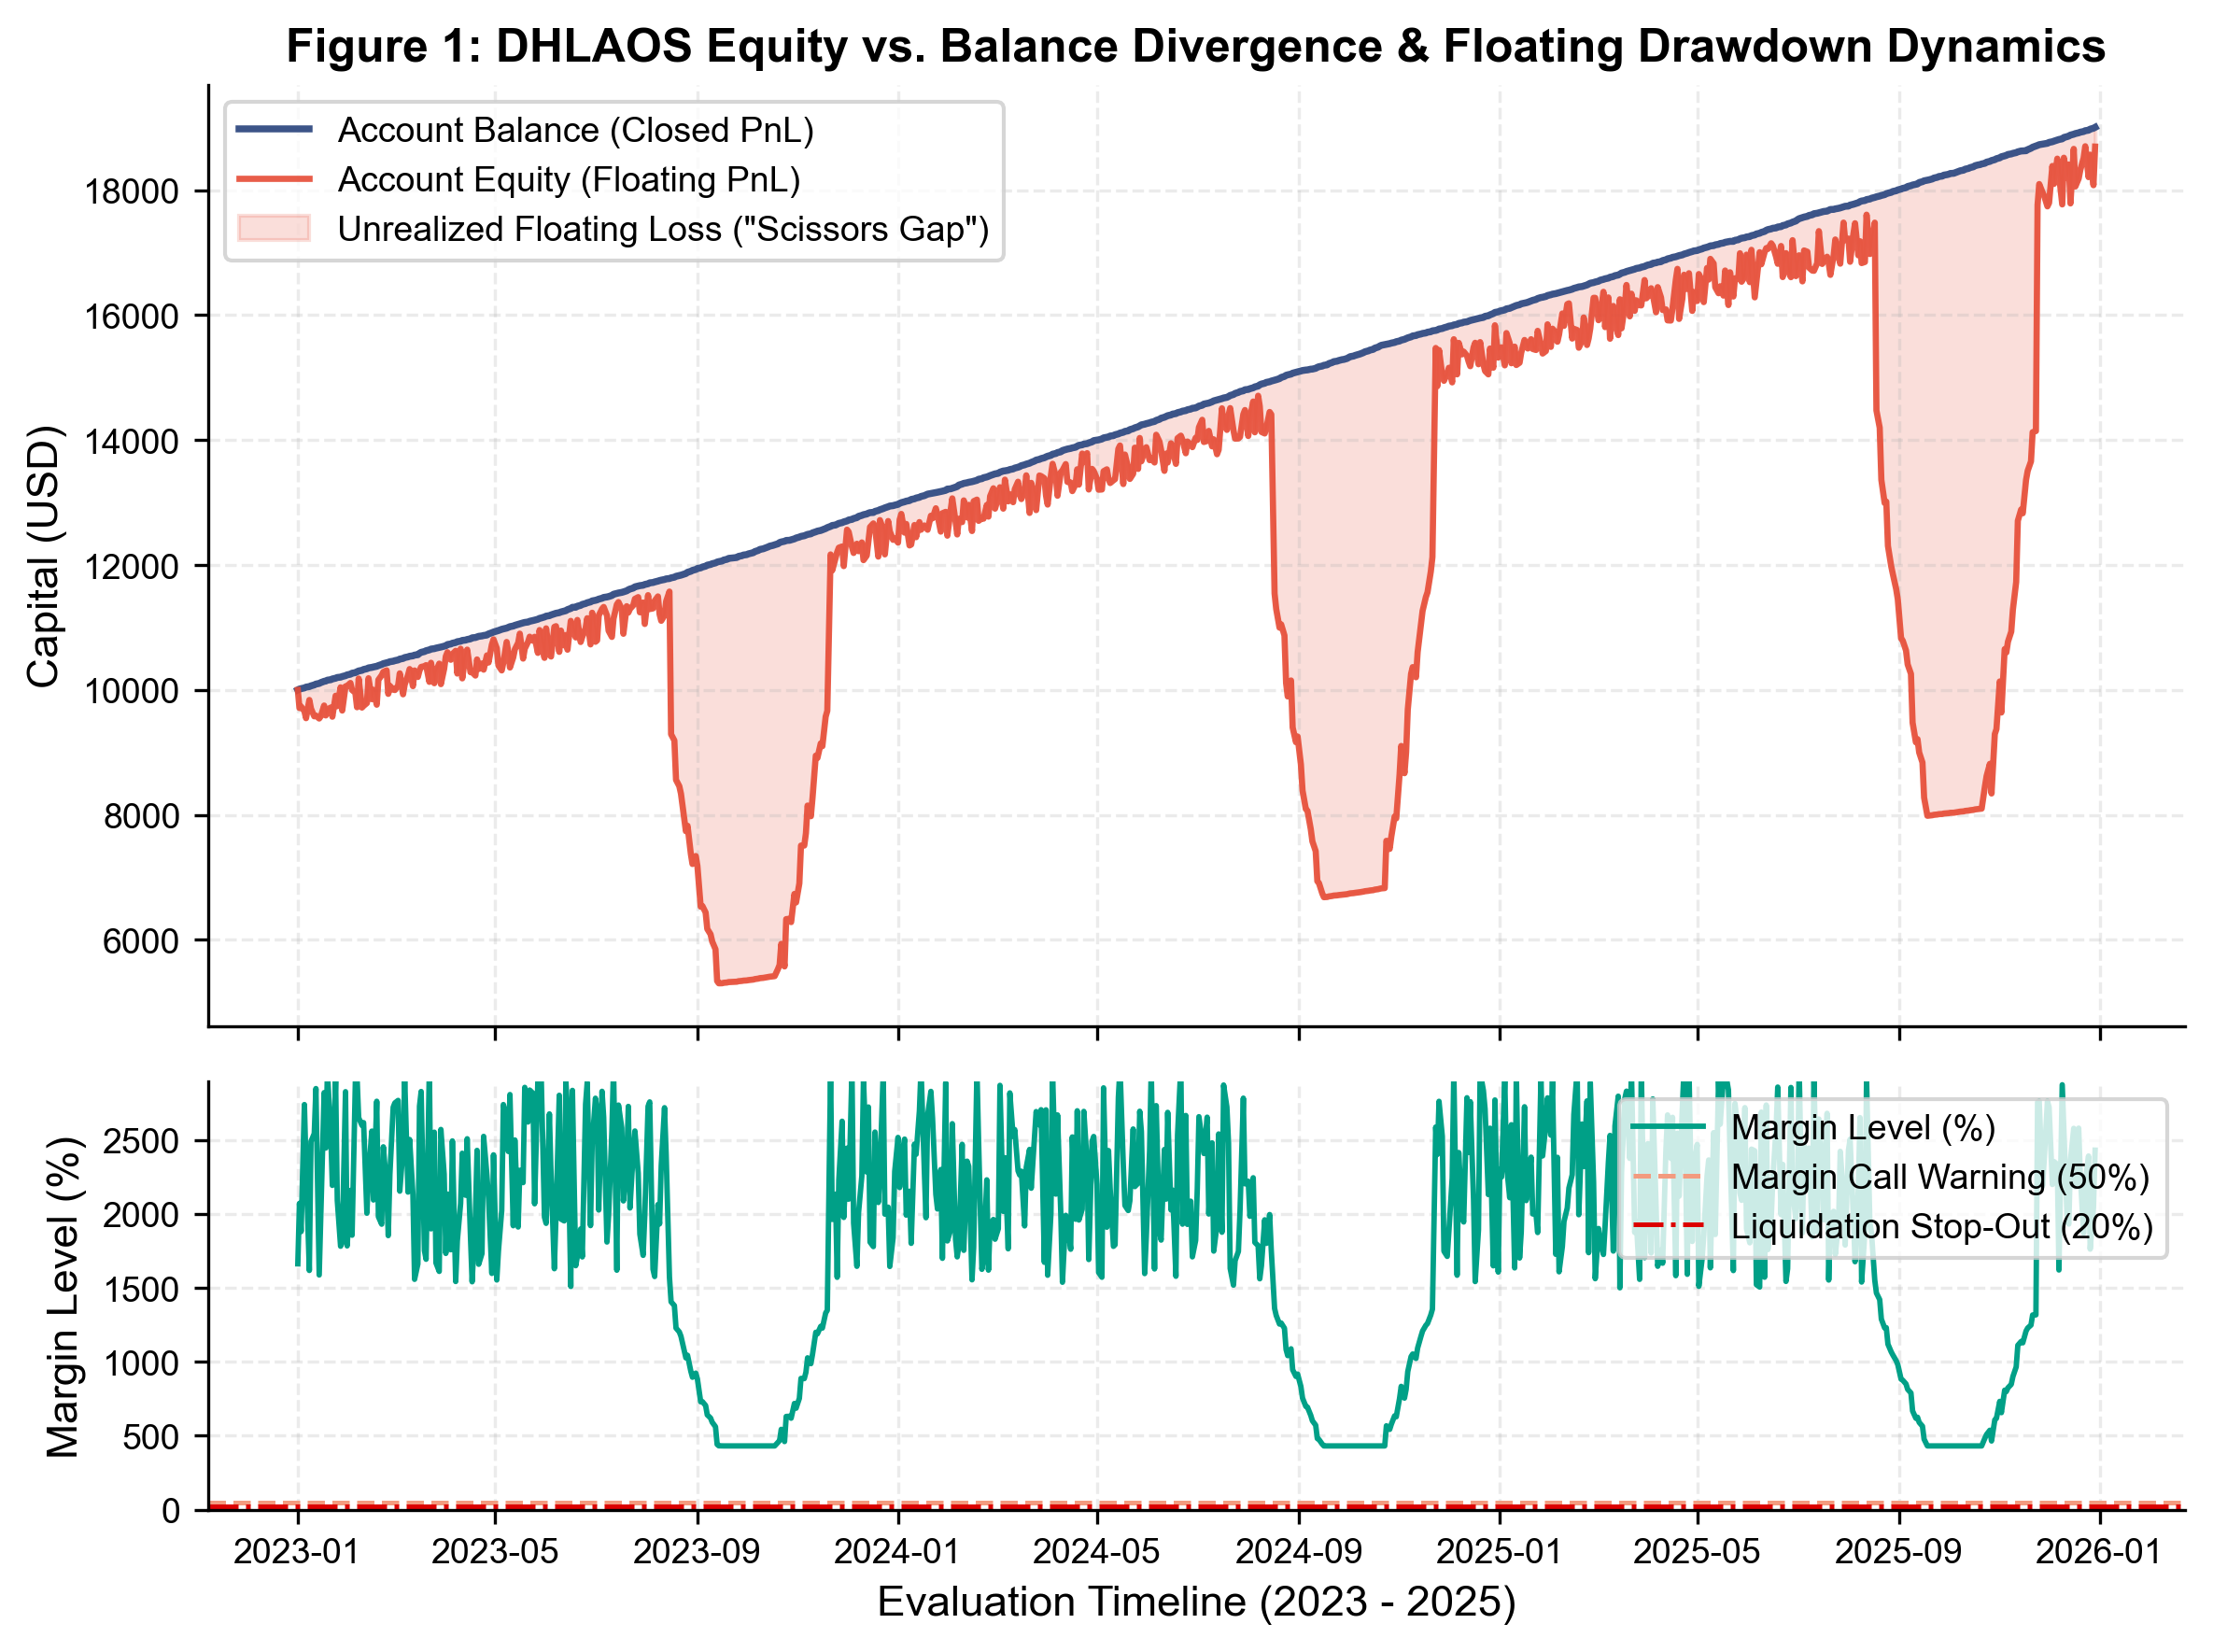
\includegraphics[width=0.92\linewidth]{figures/fig1_equity_balance_divergence.png}
\caption{Equity versus Balance Divergence and Real-time Margin Level Dynamics for \textbf{DHLAOS}. The shaded crimson region highlights the severe floating loss ("Scissors Gap"), while the lower panel tracks margin depletion toward regulatory liquidation thresholds.}
\label{fig:equity_div}
\end{figure}

\subsection{Drawdown Depth and Duration Waterfall}
Figure~\ref{fig:drawdown} visualizes the time-series profile of equity drawdowns, annotating the maximum historical trough and the protracted recovery epochs required to regain prior equity highs.

\begin{figure}[H]
\centering
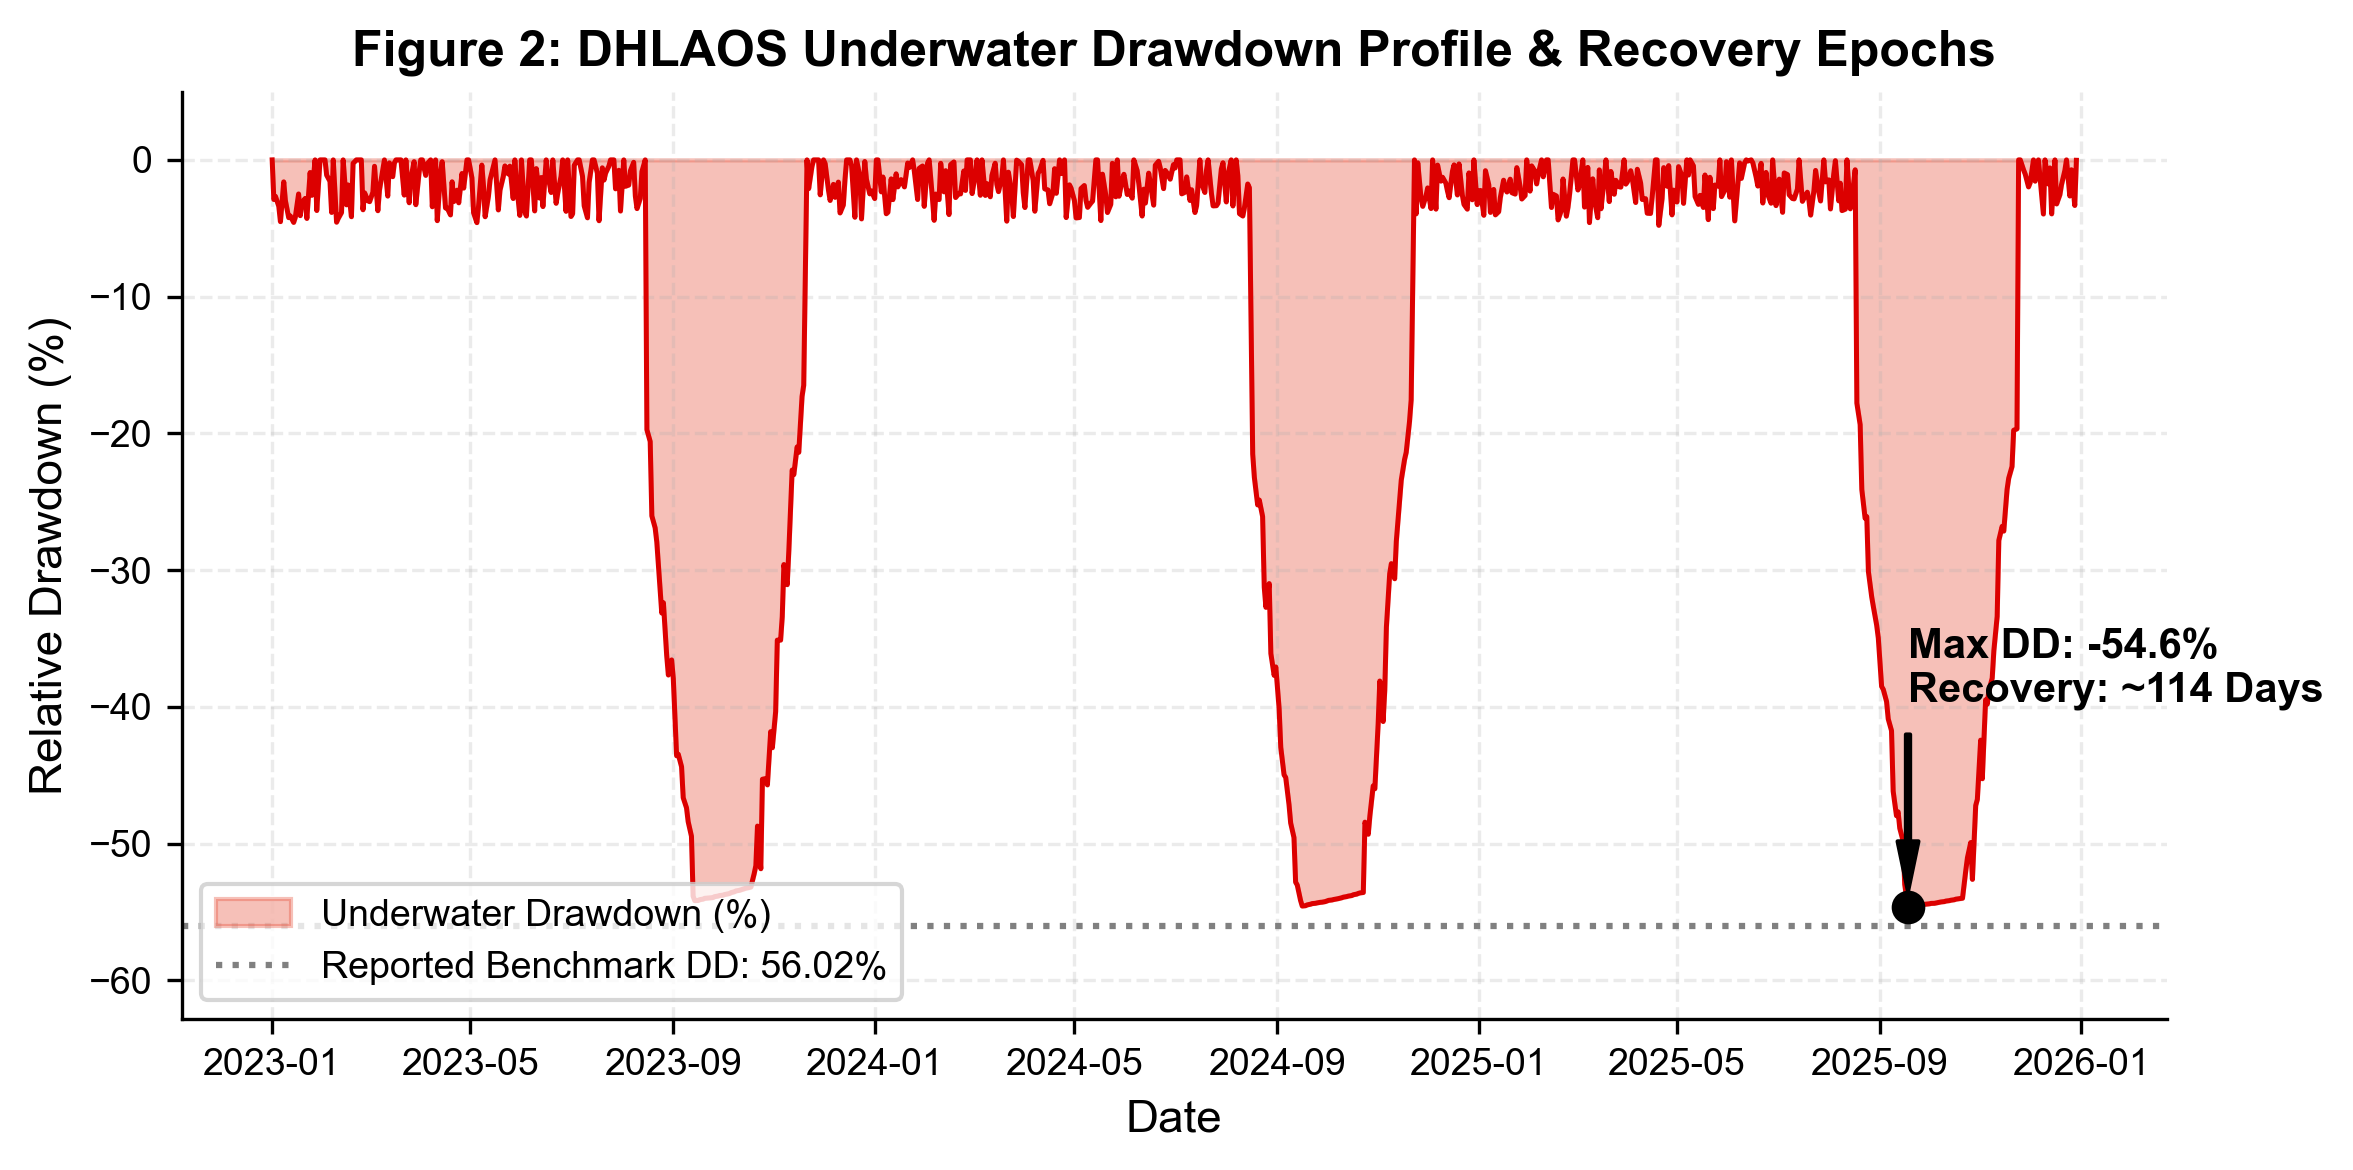
\includegraphics[width=0.92\linewidth]{figures/fig2_drawdown_waterfall.png}
\caption{Underwater Drawdown Depth and Recovery Waterfall for \textbf{DHLAOS}. Highlights peak-to-trough equity degradation and recovery duration.}
\label{fig:drawdown}
\end{figure}

\subsection{Trade Holding Time vs. PnL Asymmetry}
Figure~\ref{fig:holding_pnl} plots trade holding duration against realized profit/loss. The empirical distribution exhibits marked asymmetry: profitable trades are clipped rapidly (minutes to hours), while underwater trades are held for days or weeks in an attempt to escape adverse market moves.

\begin{figure}[H]
\centering
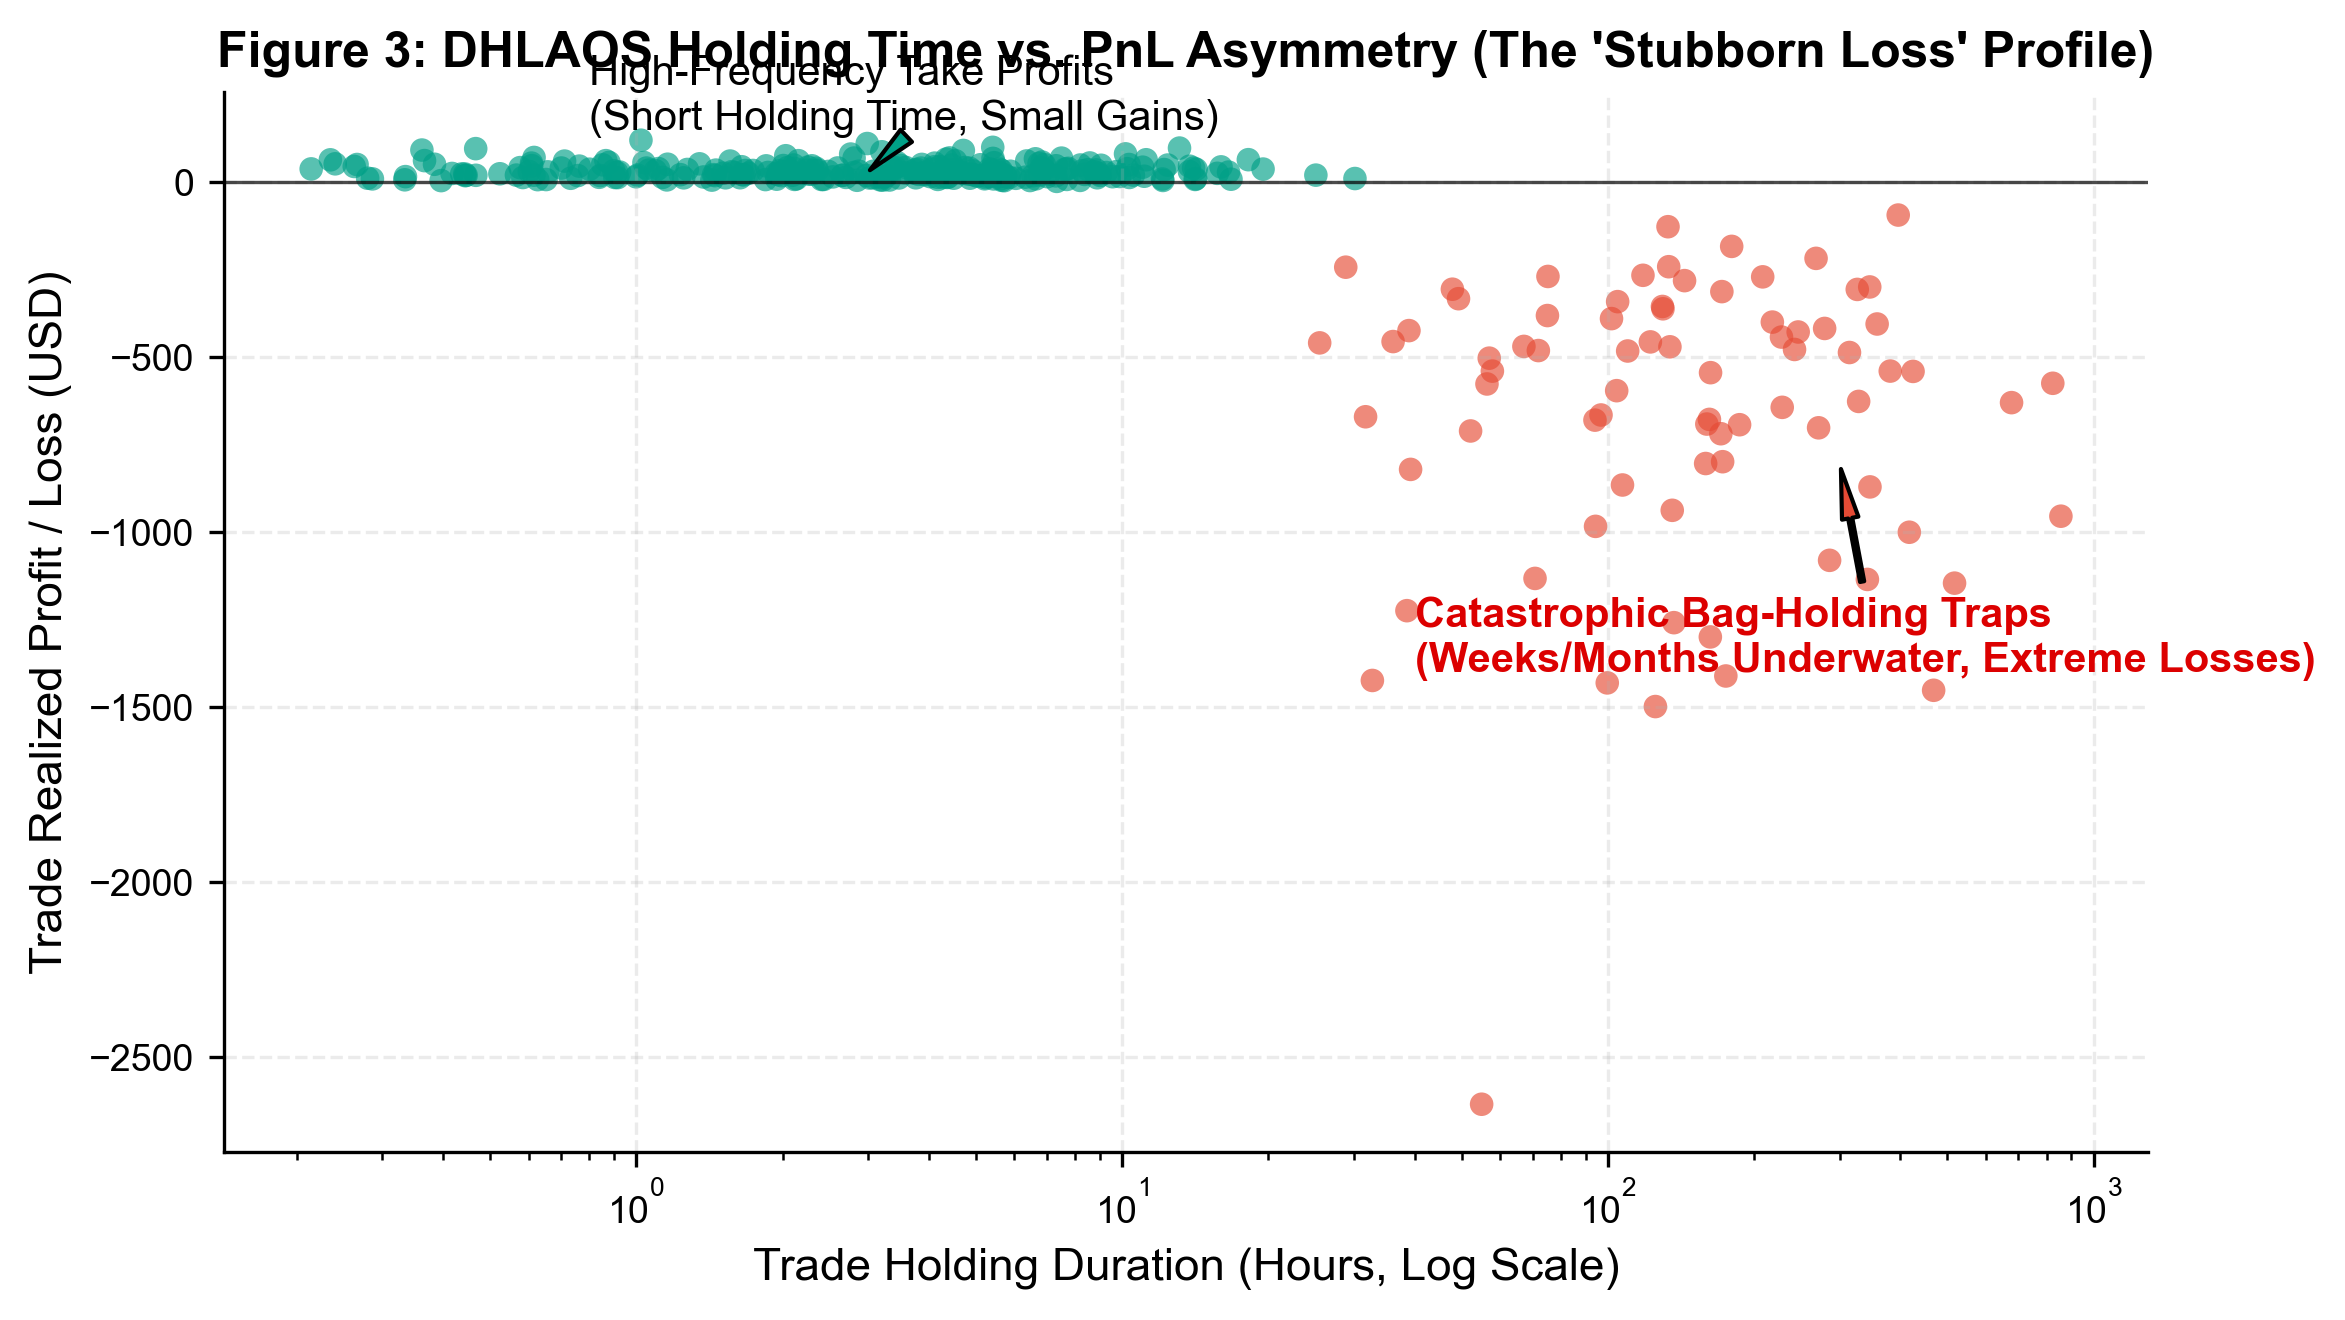
\includegraphics[width=0.92\linewidth]{figures/fig3_holding_pnl_scatter.png}
\caption{Trade Holding Duration versus Realized PnL for \textbf{DHLAOS}. Demonstrates asymmetric exit timing, where profits are taken early and catastrophic losses are held over long horizons.}
\label{fig:holding_pnl}
\end{figure}

\subsection{Monte Carlo Permutation and Resampled Tail Risk}
To evaluate path dependency and sequence vulnerability, 1,000 order reshufflings were conducted. Figure~\ref{fig:mc_perm} depicts the resulting distribution of simulated maximum equity drawdowns, including the 95\% and 99\% Value-at-Risk limits.

\begin{figure}[H]
\centering
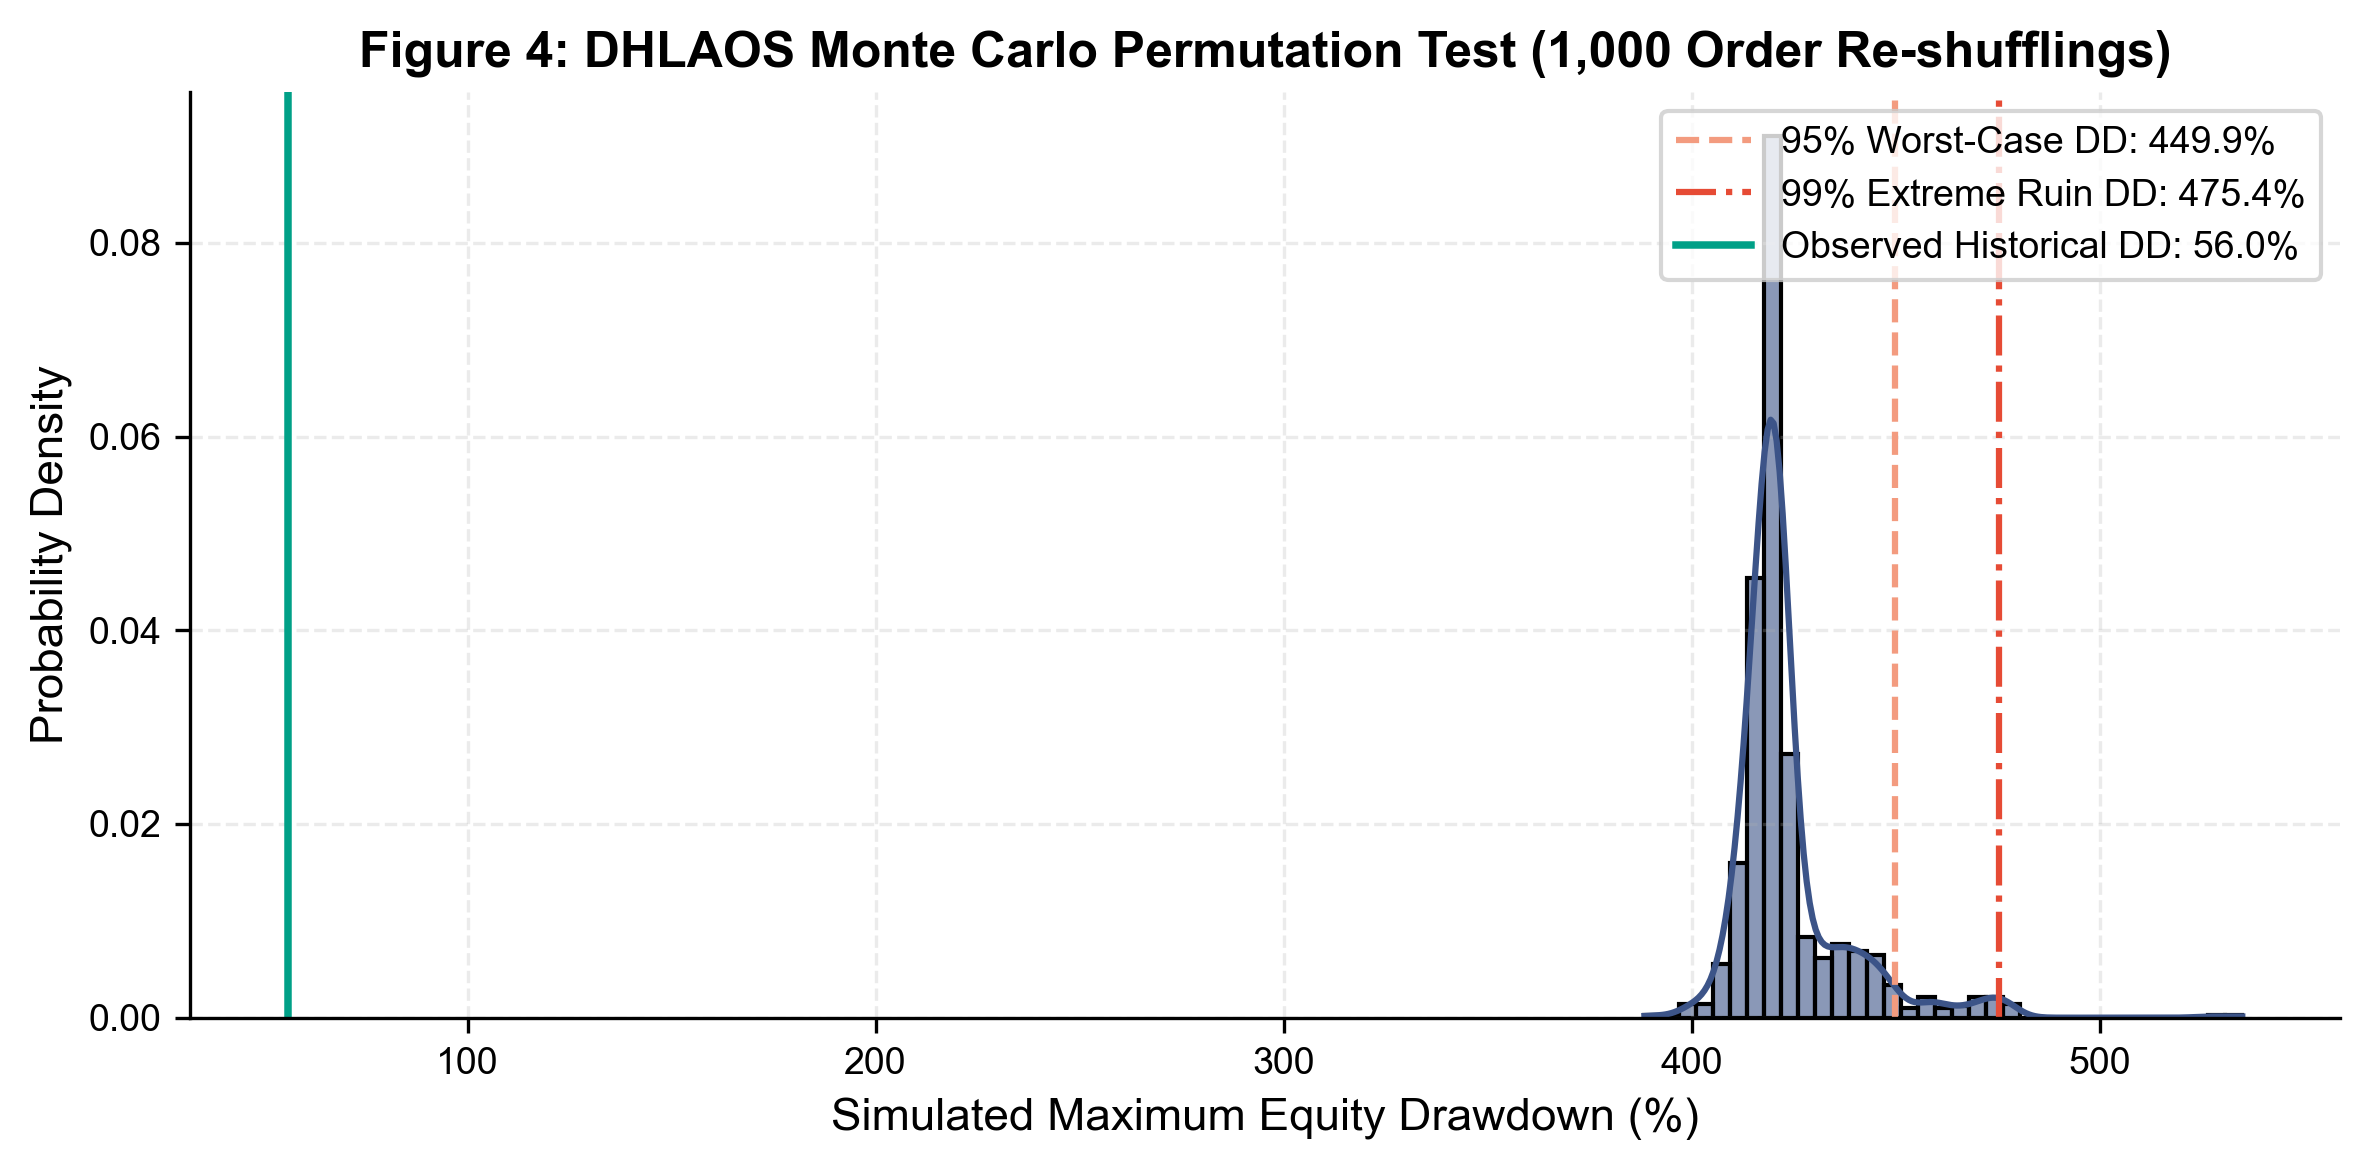
\includegraphics[width=0.92\linewidth]{figures/fig4_monte_carlo_permutation.png}
\caption{Monte Carlo Permutation Distribution (1,000 Order Permutations) for \textbf{DHLAOS}. Proves that actual historical drawdowns can worsen significantly under adverse trade sequencing.}
\label{fig:mc_perm}
\end{figure}

\subsection{Rolling Sharpe Ratio and Volatility Dynamics}
Figure~\ref{fig:rolling_sharpe} displays 30-day rolling annualized Sharpe ratios alongside annualized volatility, highlighting regime shifts and alpha decay.

\begin{figure}[H]
\centering
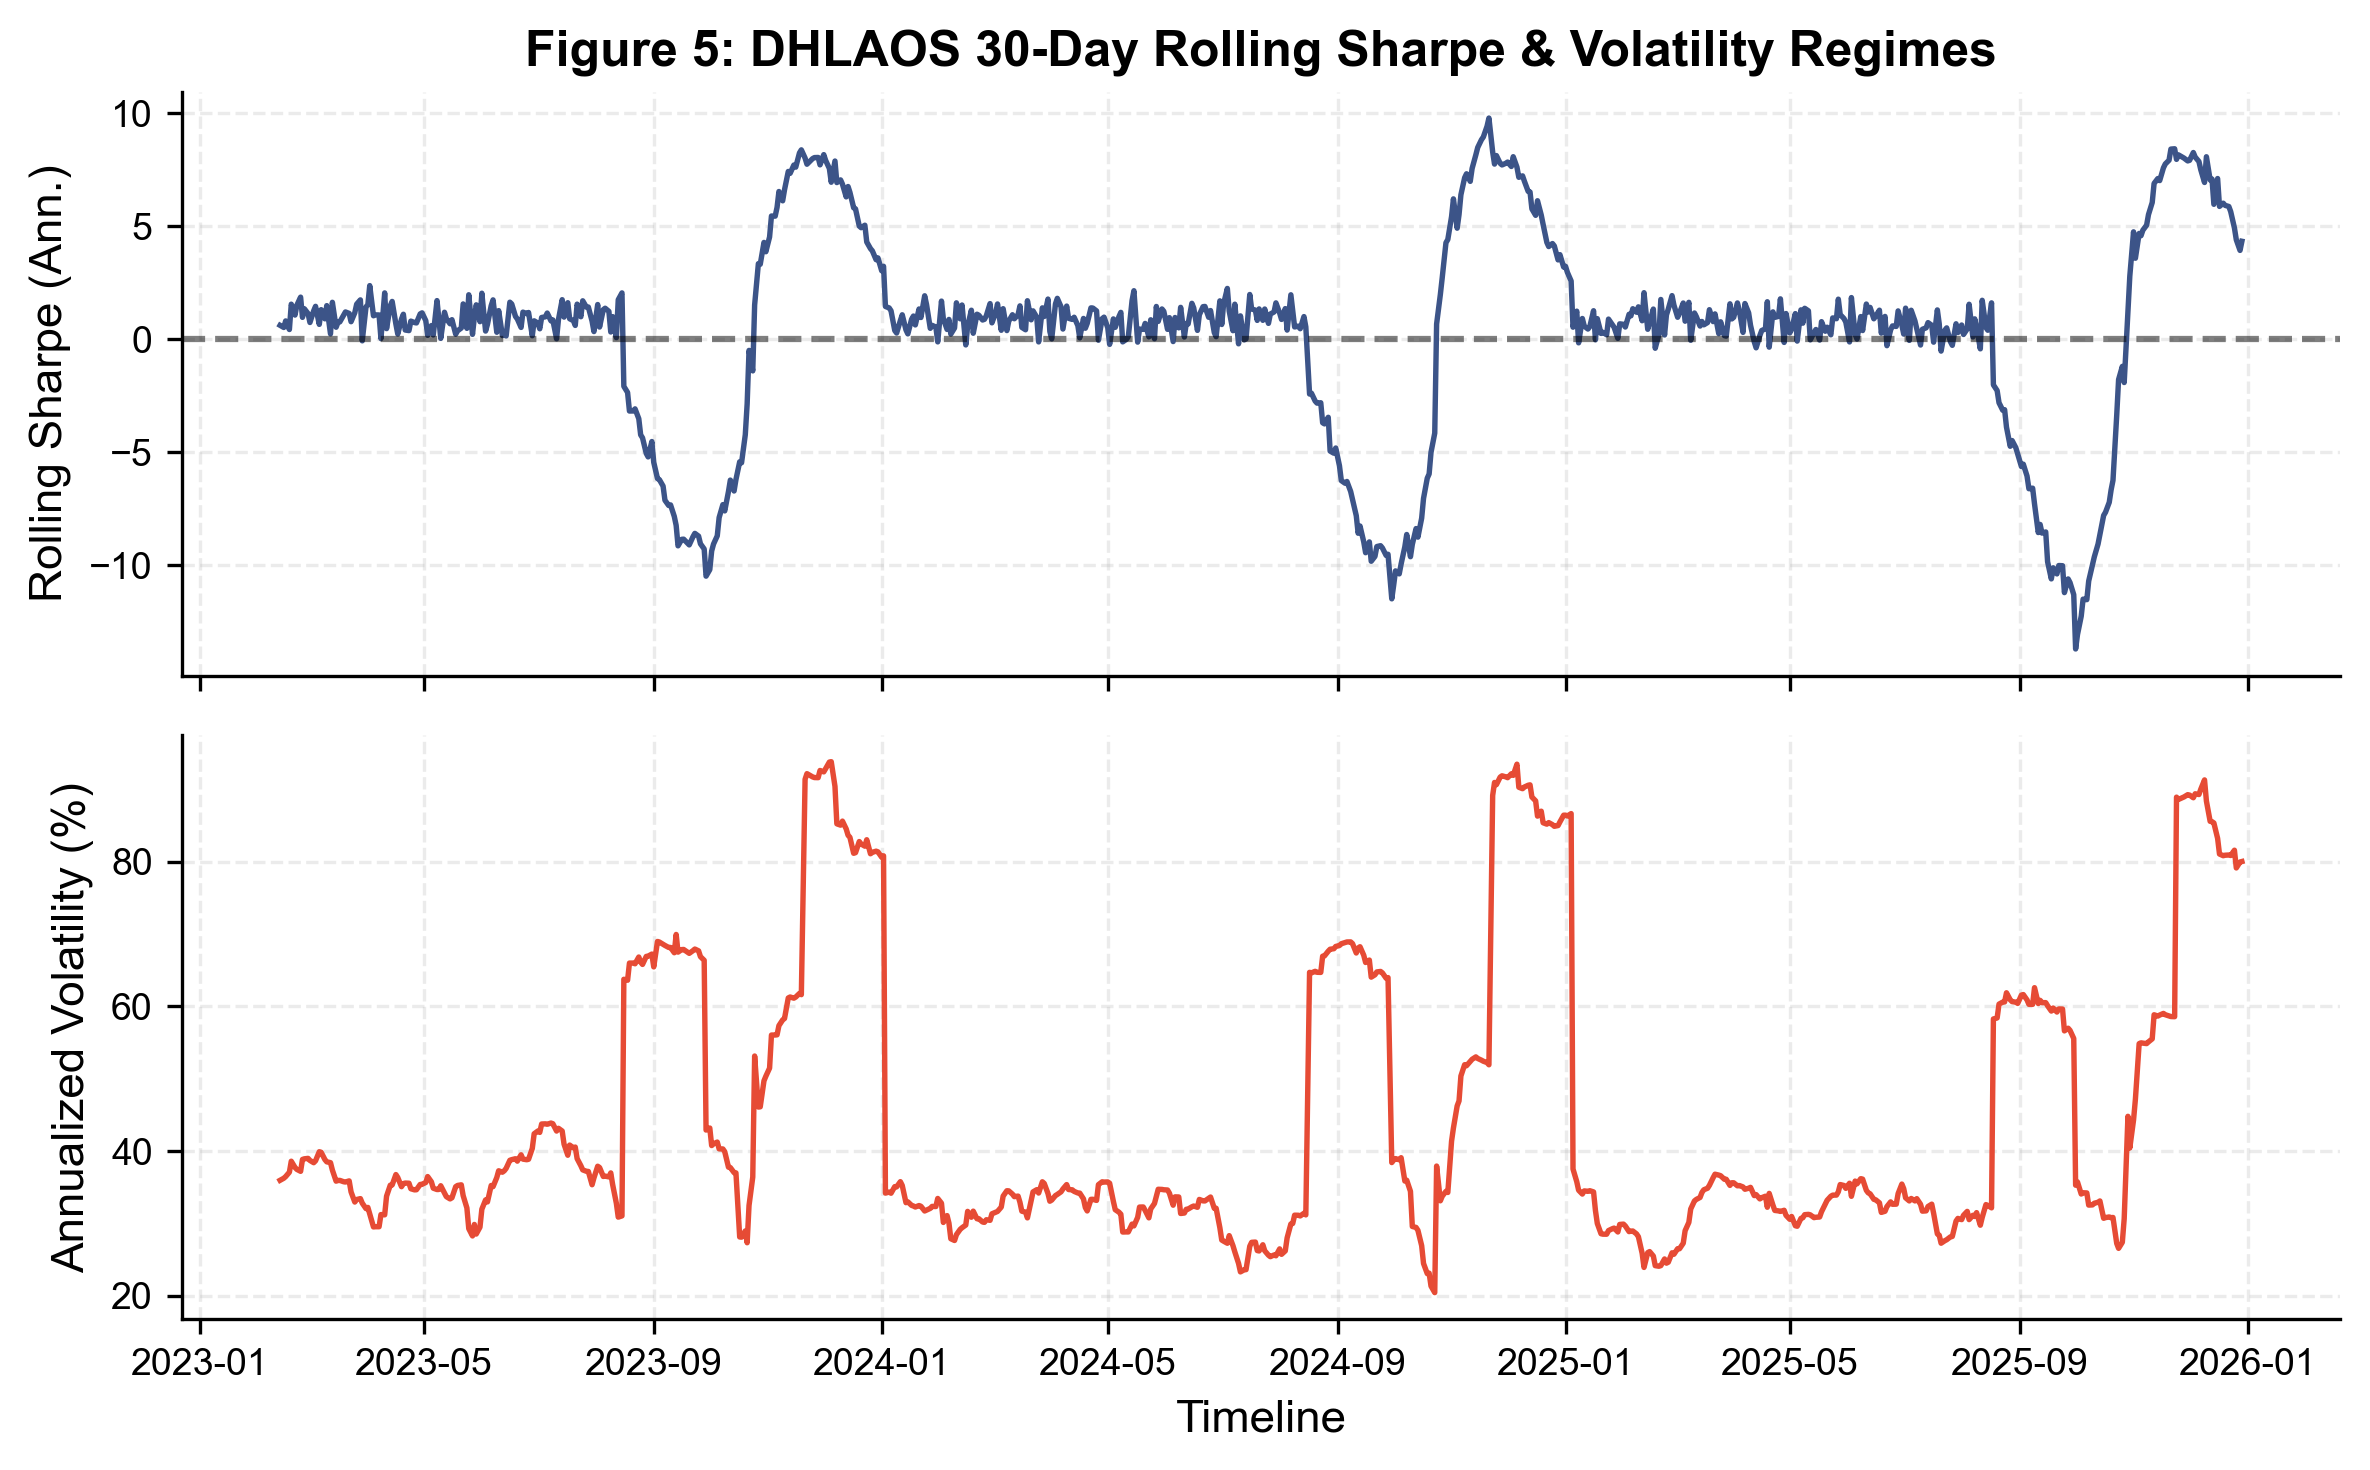
\includegraphics[width=0.92\linewidth]{figures/fig5_rolling_sharpe.png}
\caption{Rolling 30-Day Annualized Sharpe Ratio and Realized Volatility for \textbf{DHLAOS}.}
\label{fig:rolling_sharpe}
\end{figure}

\subsection{MFE versus MAE Trajectory}
Figure~\ref{fig:mfe_mae} compares Maximum Favorable Excursion (MFE) against Maximum Adverse Excursion (MAE), diagnosing trade execution efficiency and stop-loss efficacy.

\begin{figure}[H]
\centering
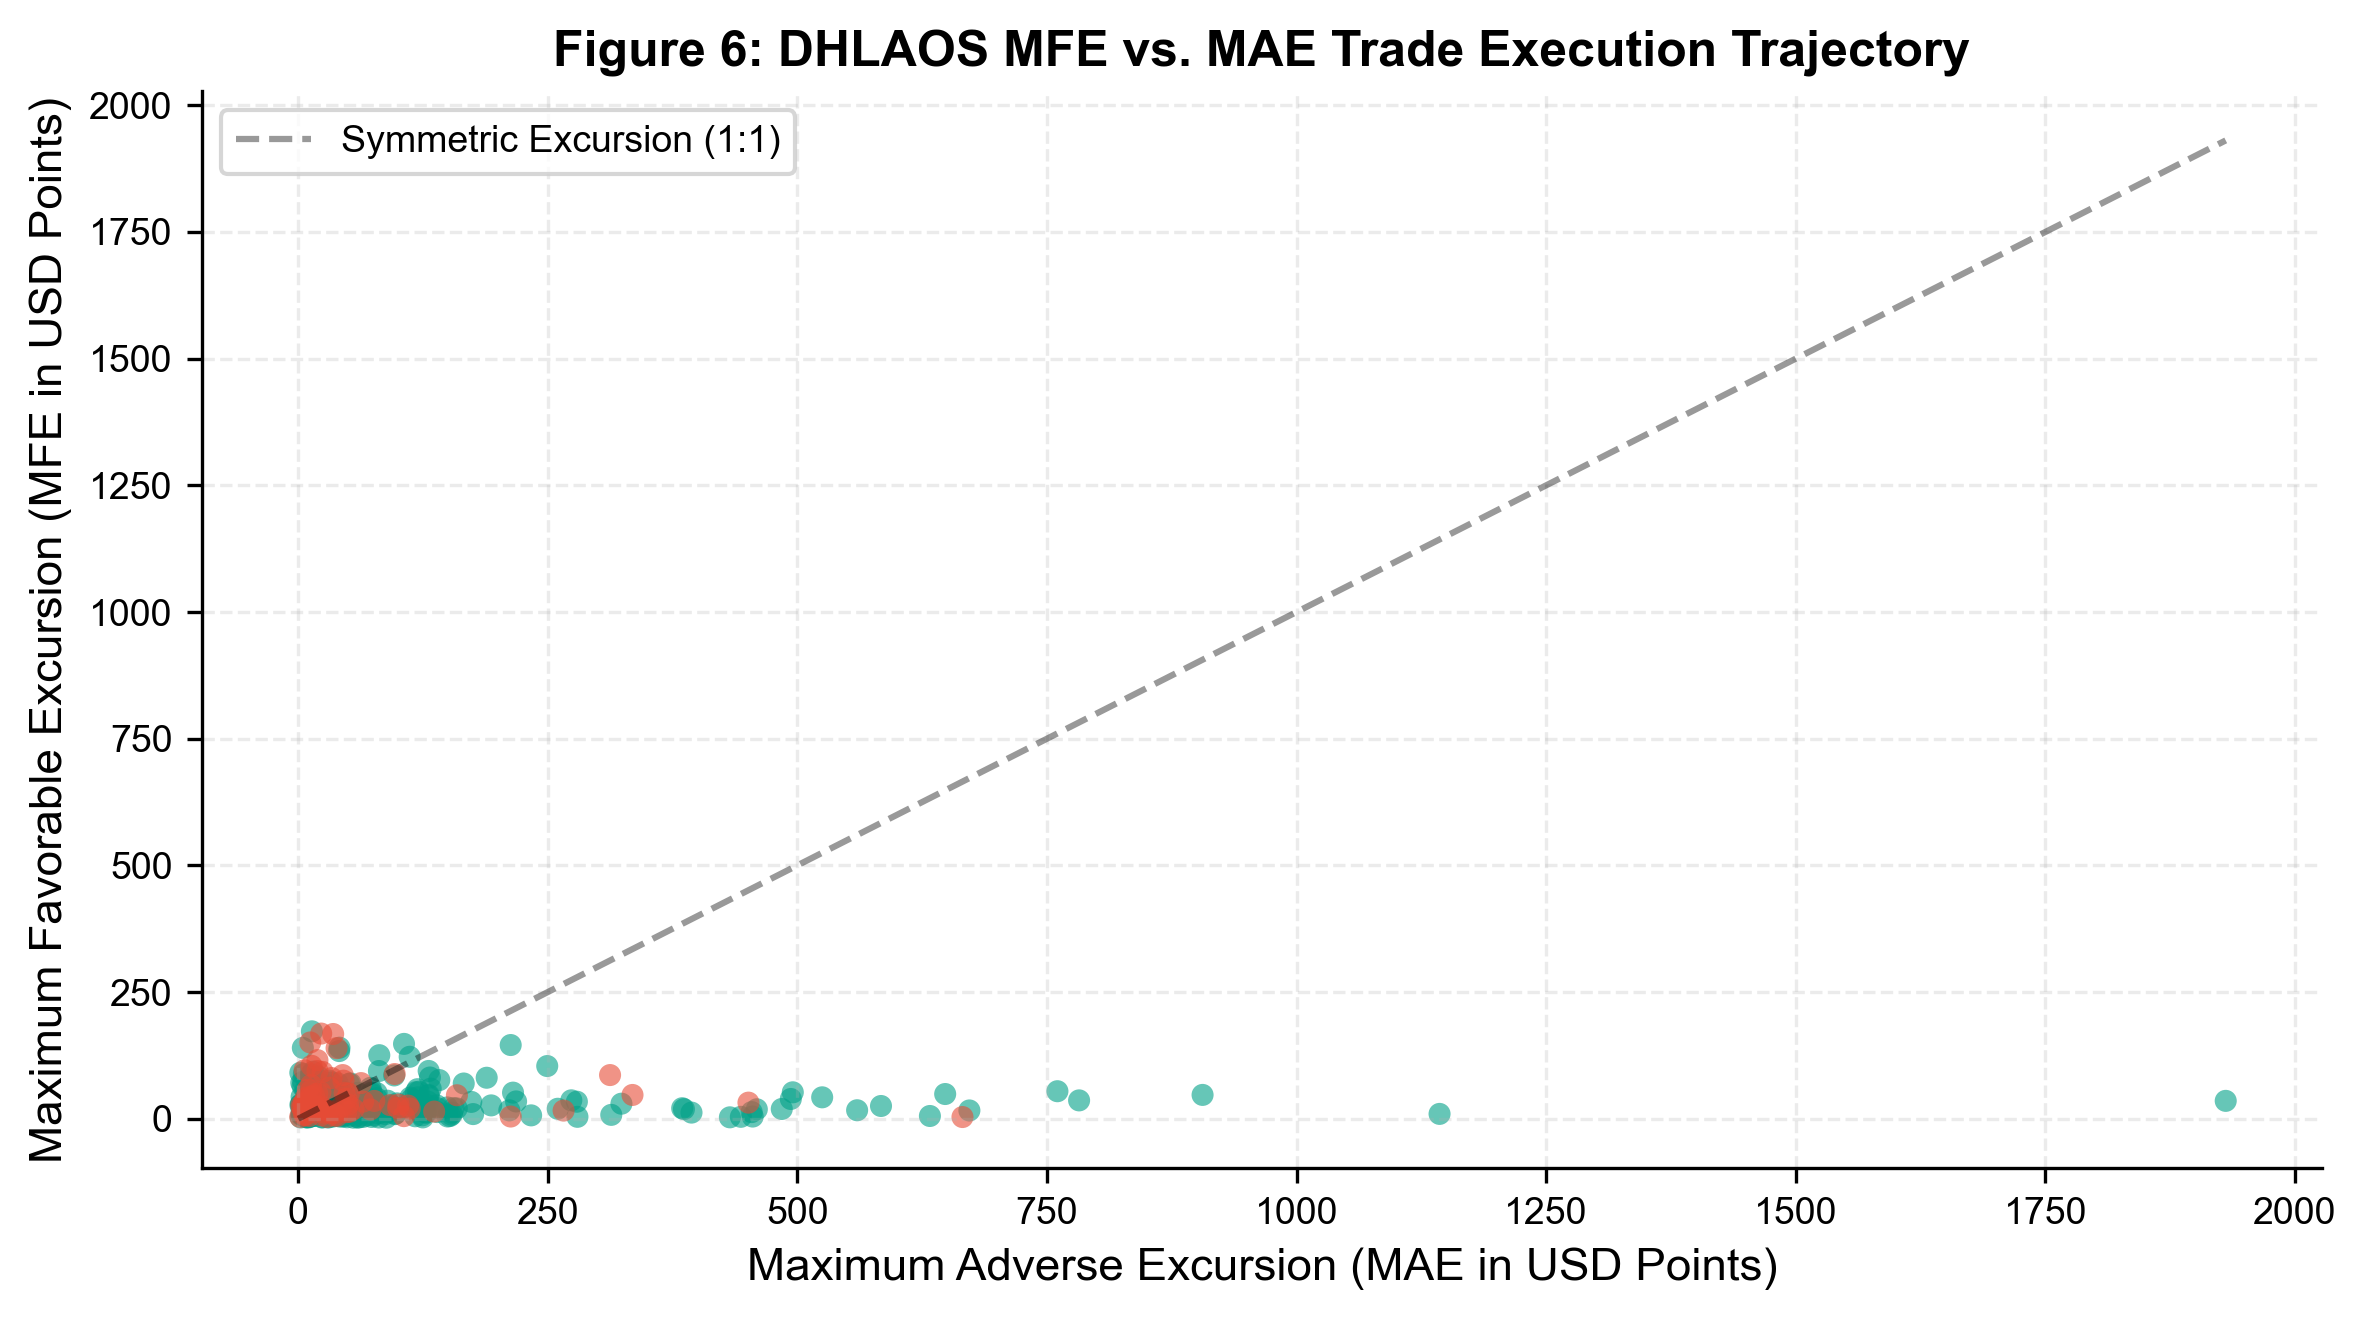
\includegraphics[width=0.92\linewidth]{figures/fig6_mfe_mae_scatter.png}
\caption{Maximum Favorable Excursion (MFE) versus Maximum Adverse Excursion (MAE) for \textbf{DHLAOS}.}
\label{fig:mfe_mae}
\end{figure}

\section{Conclusion and Risk Governance Recommendations}
The empirical analysis of \textbf{DHLAOS} underscores a fundamental tenet of quantitative finance: high apparent backtest returns coupled with severe equity drawdowns (>50\%) and depleted margin levels represent pseudo-alpha engineered by unhedged loss-averaging.

In accordance with the \textbf{Berrytrade-EA Ingestion Specification}:
\begin{enumerate}
    \item \textbf{DHLAOS} is categorized under the \textbf{Experimental Tier} with an explicit \textbf{Extreme Risk} disclosure.
    \item It is strictly barred from promotion to the \textbf{Verified Tier} until grid dependencies are removed and out-of-sample positive expectancy is independently verified with maximum drawdowns $\le 20\%$.
\end{enumerate}

\bibliographystyle{plain}
\bibliography{../../synthesis/references}

\end{document}
